\documentclass[12pt, a4paper]{article}
\usepackage[utf8]{inputenc}
\usepackage[T1]{fontenc}
\usepackage{lmodern}
\usepackage[english]{babel}
\usepackage{microtype}
\usepackage{geometry}
\geometry{a4paper, margin=1in}
\usepackage{graphicx}
\usepackage{float}
\usepackage{hyperref}
\usepackage{fancyhdr}
\usepackage{setspace}
\usepackage{listings}
\usepackage{xcolor}
\usepackage{booktabs}
\usepackage{array}
\usepackage{enumitem}
\usepackage{mdframed}
\usepackage{cite}

\hypersetup{
    colorlinks=true,
    linkcolor=blue,
    filecolor=magenta,
    urlcolor=cyan,
    pdftitle={Project Report: ORION},
}

\lstdefinestyle{mystyle}{
    backgroundcolor=\color{gray!10},
    commentstyle=\color{green!50!black},
    keywordstyle=\color{blue},
    numberstyle=\tiny\color{gray},
    stringstyle=\color{purple},
    basicstyle=\ttfamily\footnotesize,
    breakatwhitespace=false,
    breaklines=true,
    captionpos=b,
    keepspaces=true,
    numbers=left,
    numbersep=5pt,
    showspaces=false,
    showstringspaces=false,
    showtabs=false,
    tabsize=2
}
\lstset{style=mystyle}

\pagestyle{fancy}
\fancyhf{}
\fancyhead[L]{\small ORION: Multi-Agent Deep Research Platform}
\fancyhead[R]{\small PCCOE, Pune}
\fancyfoot[C]{\thepage}
\renewcommand{\headrulewidth}{0.4pt}

\begin{document}

%----------------------------------------------------------------------------------------
%  1. TITLE PAGE
%----------------------------------------------------------------------------------------
\begin{titlepage}
    \begin{center}
        \noindent\rule{\textwidth}{2pt}
        \vspace{0.3cm}

        {\large \textbf{Pimpri Chinchwad College of Engineering (PCCOE), Pune}}\\
        \vspace{0.1cm}
        {\normalsize Department of Computer Science and Engineering (AI \& ML)}\\
        \vspace{0.1cm}
        {\normalsize Academic Year: 2025--2026}

        \vspace{0.2cm}
        \noindent\rule{\textwidth}{1pt}
        \vspace{1.2cm}

        {\Large \textbf{Elective Project Work Report}}\\
        \vspace{0.3cm}
        {\small (Third Year B.Tech --- CSE (AI \& ML))}

        \vspace{1.4cm}

        \begin{mdframed}[linewidth=1.5pt, innertopmargin=12pt, innerbottommargin=12pt]
            \centering
            \LARGE \textbf{Multi-Agent Deep Research Platform}\\[6pt]
            \Large \textbf{(ORION)}
        \end{mdframed}

        \vspace{1.6cm}

        \renewcommand{\arraystretch}{1.4}
        \begin{tabular}{|c|l|l|}
            \hline
            \textbf{Sr. No.} & \textbf{Student Name} & \textbf{PRN} \\
            \hline
            1 & Vikram Kadam   & 123B1C013 \\
            2 & Keshav Mittal  & 123B1C015 \\
            3 & Sandesh Phad   & 123B1C033 \\
            4 & Tejas Shidam   & 123B1C037 \\
            \hline
        \end{tabular}

        \vspace{1.5cm}

        \begin{tabular}{ll}
            \textbf{Project Guide:} & Mrs.\ Madhuri Pagale \\
        \end{tabular}

        \vfill
        \noindent\rule{\textwidth}{2pt}
    \end{center}
\end{titlepage}

\newpage
\pagenumbering{roman}

%----------------------------------------------------------------------------------------
%  2. ABSTRACT
%----------------------------------------------------------------------------------------
\section*{Abstract}
\addcontentsline{toc}{section}{Abstract}

The process of conducting a comprehensive academic literature review is traditionally a manual,
time-consuming task prone to human bias and oversight. As the volume of scientific literature
grows exponentially, researchers struggle to efficiently synthesize findings, identify genuine
contradictions, and pinpoint viable research gaps.

To address this challenge, we present the \textbf{Multi-Agent Deep Research Platform (ORION)},
an automated, LLM-powered orchestration framework. ORION employs a sophisticated
\textbf{LangGraph-based multi-agent architecture} that autonomously plans search queries,
retrieves peer-reviewed papers from multiple academic databases (Semantic~Scholar, Crossref,
ArXiv), extracts structured metrics, and conducts rigorous cross-paper analysis.

A distinguishing feature of ORION is its \textbf{adversarial Critic-Proposer debate mechanism},
which iteratively vets generated claims to significantly reduce hallucinations and achieve high
citation grounding accuracy. This reduces the time required for initial literature surveys from
days to minutes, producing comprehensive, fully cited research dossiers and visually rich
analytical reports.

\vspace{0.5cm}
\noindent\textbf{Keywords:} Multi-Agent Systems, LangGraph, Large Language Models,
Literature Review Automation, Research Gap Analysis, Retrieval-Augmented Generation,
Adversarial Debate.

\newpage

%----------------------------------------------------------------------------------------
%  3. TABLE OF CONTENTS
%----------------------------------------------------------------------------------------
\tableofcontents
\newpage
\pagenumbering{arabic}
\onehalfspacing

%----------------------------------------------------------------------------------------
%  4. INTRODUCTION
%----------------------------------------------------------------------------------------
\section{Introduction}

\subsection{Background}
The scientific method fundamentally depends on a thorough understanding of existing work
before new hypotheses can be proposed. Researchers today face an overwhelming influx of
publications across disciplines, with millions of new papers published annually. Manually
extracting quantitative metrics, mapping methodological differences, and synthesizing debates
across dozens of papers requires substantial time and cognitive effort that detracts from
actual research contributions.

Large Language Models (LLMs) have demonstrated strong capabilities in text comprehension
and synthesis \cite{brown2020gpt}. However, deploying them reliably for academic tasks
requires careful orchestration to prevent factual errors and fabricated citations --- a
well-documented limitation of single-prompt LLM pipelines \cite{ji2023hallucination}.
Multi-agent frameworks, where specialized agents collaborate on sub-tasks, have emerged as
a promising solution to this problem \cite{wu2023autogen}.

\subsection{Problem Statement}
Existing literature survey tools either function as simple semantic search engines or generate
summaries without verifiable citations and deep cross-paper analysis. There is a critical lack
of autonomous systems capable of reading multiple papers in-depth, identifying contradictions
and agreements, and proposing structured, actionable research gaps in a format immediately
usable by academic and industrial R\&D teams. Furthermore, general-purpose LLMs are prone
to hallucination, producing fabricated citations that undermine research integrity
\cite{ji2023hallucination}.

\subsection{Objectives}
\begin{itemize}[leftmargin=*, itemsep=3pt]
    \item Develop a multi-agent system capable of retrieving and deeply analyzing scientific
          literature from heterogeneous academic databases.
    \item Implement a robust validation pipeline (Critic-Proposer adversarial debate) to
          significantly reduce hallucinations and achieve high citation grounding accuracy.
    \item Generate structured, publication-style literature reviews with integrated visual
          gap-analysis dossiers.
    \item Provide a dynamic, real-time web interface for users to monitor the agentic
          workflow and interact with the generated research.
    \item Enable private corpus integration via PDF upload and vector store grounding.
\end{itemize}

%----------------------------------------------------------------------------------------
%  5. LITERATURE SURVEY
%----------------------------------------------------------------------------------------
\section{Literature Survey}

\subsection{Related Work}

The landscape of AI-assisted research tools has evolved rapidly. We review three major
categories of prior work below.

\textbf{Semantic Search and Question-Answering Systems.}
Tools such as Elicit \cite{elicit2023} and Consensus apply semantic similarity models to
retrieve and cluster relevant papers. While effective for targeted fact-finding, these systems
return isolated answer snippets rather than synthesizing a comprehensive, multi-section
literature review that maps methodological patterns or identifies research trajectories.

\textbf{Retrieval-Augmented Generation (RAG).}
Lewis et al.\ \cite{lewis2020rag} introduced RAG as a method to ground LLM outputs in
retrieved documents, substantially reducing hallucination rates compared to closed-book
generation. ORION adopts RAG principles at its retrieval and summarization stages, extending
them with per-source citation verification and confidence metadata.

\textbf{Multi-Agent LLM Frameworks.}
Wu et al.\ \cite{wu2023autogen} proposed AutoGen, demonstrating that decomposing complex
tasks across collaborating LLM agents improves output reliability. Similarly, Hong et al.\
\cite{hong2023metagpt} introduced MetaGPT, which assigns structured roles to agents within
a software development workflow. ORION adapts these principles specifically for the academic
review domain, introducing an adversarial peer-review node and structured gap analysis within
a deterministic state-machine graph.

\textbf{Hallucination in LLMs.}
Ji et al.\ \cite{ji2023hallucination} conducted a systematic survey of hallucination in natural
language generation, identifying citation fabrication as a critical risk in knowledge-intensive
tasks. ORION directly addresses this through its Critic agent, which audits every claim in the
draft against retrieved source keys before approving the output.

\subsection{Comparative Analysis}

\vspace{0.3cm}
\renewcommand{\arraystretch}{1.5}
\begin{tabular}{|p{3.5cm}|p{4.2cm}|p{5.2cm}|}
    \hline
    \textbf{System} & \textbf{Strengths} & \textbf{Limitations} \\
    \hline
    Elicit / Consensus \cite{elicit2023}
        & Accurate semantic search; fast answers
        & No multi-page synthesis; no methodology mapping \\
    \hline
    ChatGPT / Claude (closed-book)
        & Fluent summarization; broad coverage
        & High hallucination rate; no live retrieval \cite{ji2023hallucination} \\
    \hline
    AutoGen \cite{wu2023autogen}
        & Flexible multi-agent collaboration
        & Not tailored to academic review; no adversarial citation validation \\
    \hline
    RAG pipelines \cite{lewis2020rag}
        & Grounded generation; reduced hallucination
        & Single-stage; no iterative critic or gap analysis \\
    \hline
    \textbf{ORION (Proposed)}
        & Full 8-stage pipeline; adversarial validation; structured gap analysis
        & Dependent on source API availability and LLM quality \\
    \hline
\end{tabular}

%----------------------------------------------------------------------------------------
%  6. METHODOLOGY
%----------------------------------------------------------------------------------------
\section{Methodology}

\subsection{Overall Approach}
ORION adopts a deterministic, graph-based workflow modeled as a finite state machine using
LangGraph \cite{langgraph2024}. The pipeline is decomposed into eight modular agent nodes,
each responsible for a distinct cognitive sub-task. This separation of concerns ensures that
each stage can be independently monitored and improved without cascading failures.

\subsection{Pipeline Architecture}

The complete execution sequence is as follows:

\vspace{0.4cm}
\begin{center}
\small
\texttt{Planner $\rightarrow$ Retriever $\rightarrow$ Summarizer $\rightarrow$ Proposer
$\leftrightarrow$ Critic (loop) $\rightarrow$ Cross-Paper Analyzer $\rightarrow$
Gap Analyzer $\rightarrow$ Paper Architect $\rightarrow$ END}
\end{center}
\vspace{0.4cm}

\noindent The eight agent nodes and their roles are:

\begin{enumerate}[leftmargin=*, itemsep=4pt]
    \item \textbf{Search Planner:} Analyzes the user's topic and generates 3--5 distinct,
          non-overlapping search queries with quality constraints (phrase anchoring, domain
          narrowing terms, lexical overlap checks).

    \item \textbf{Retriever:} Fetches paper metadata and full-text chunks from ArXiv,
          Semantic~Scholar, Tavily, and ChromaDB (for user-uploaded PDFs). Applies
          token-overlap-based relevance scoring against the topic and query terms, and
          removes near-duplicate entries by comparing titles and DOI fields.

    \item \textbf{Summarizer:} Processes each retrieved paper into a structured JSON object
          containing the summary, methodology, core findings, limitations, and a citation
          confidence flag derived from the availability of DOI, author, and venue metadata.

    \item \textbf{Proposer (Literature Reviewer):} Drafts the initial literature review
          synthesis from the structured summaries, operating in evidence-grounded mode where
          each claim must reference a specific source key from the retrieved corpus.

    \item \textbf{Critic (Peer Reviewer):} Audits the proposer's draft for unsupported
          claims, imbalanced source representation, and citation inaccuracies. Produces a
          structured critique that is fed back into the debate loop.

    \item \textbf{Cross-Paper Analyzer:} After the debate concludes, synthesizes findings
          across all papers to map methodological agreements, contradictions, and emerging
          trends. Generates Mermaid.js architecture diagrams for visual representation.

    \item \textbf{Gap Analyzer:} Identifies actionable research gaps, each structured as a
          triple of (title, supporting evidence, proposed direction). Includes a JSON
          parsing and repair retry mechanism and a minimum-gap count check to ensure the
          output is substantive even on sparse corpora.

    \item \textbf{Paper Architect:} Assembles the final publication-style Markdown document.
          Applies post-processing normalization for the chosen citation format (APA, IEEE,
          ACM, or MLA), builds the bibliography, and computes a format compliance score
          based on structural and citation-style checks.
\end{enumerate}

\subsection{Critic-Proposer Debate Loop}
The debate loop is the primary reliability mechanism. After each proposer draft, the critic
evaluates it against the retrieved source corpus. If unsupported claims are found, a
structured critique is returned to the proposer, which revises the draft accordingly. This
cycle repeats for a configurable maximum of 1--5 rounds. Only a draft that passes critic
scrutiny proceeds to the cross-paper analysis stage, ensuring output quality is enforced
algorithmically rather than relying on a single LLM pass.

%----------------------------------------------------------------------------------------
%  7. TOOLS & TECHNOLOGIES
%----------------------------------------------------------------------------------------
\section{Tools \& Technologies}

\renewcommand{\arraystretch}{1.4}
\begin{tabular}{|p{3.8cm}|p{8.8cm}|}
    \hline
    \textbf{Category} & \textbf{Technology / Tool} \\
    \hline
    AI / LLM & Google Gemini 2.0 Pro / Flash via Vertex AI API \\
    \hline
    Orchestration & LangGraph \cite{langgraph2024}, LangChain \\
    \hline
    Backend Framework & Python 3.11, FastAPI, Uvicorn \\
    \hline
    Vector Database & ChromaDB (persistent, local) \\
    \hline
    Session Persistence & JSON file store + LangGraph SQLite Checkpointer \\
    \hline
    Frontend Framework & React (TypeScript), Vite, Tailwind CSS \\
    \hline
    Real-time Communication & WebSockets (FastAPI native support) \\
    \hline
    Academic Data Sources & ArXiv API, Semantic~Scholar API, Crossref API, Tavily Search API \\
    \hline
    PDF Processing & PyMuPDF (text extraction and chunking) \\
    \hline
    Diagram Rendering & Mermaid.js (client-side, in-browser rendering) \\
    \hline
\end{tabular}

%----------------------------------------------------------------------------------------
%  8. IMPLEMENTATION
%----------------------------------------------------------------------------------------
\section{Implementation}

\subsection{System Design and Module Structure}

The backend is organized as a modular FastAPI application. Key modules and their
responsibilities are as follows:

\begin{itemize}[leftmargin=*, itemsep=3pt]
    \item \textbf{\texttt{graph.py}:} Defines the LangGraph state machine --- nodes, edges,
          conditional debate routing, and entry/exit points.
    \item \textbf{\texttt{agents.py}:} Contains all prompt engineering and execution logic
          for each of the 8 agent nodes.
    \item \textbf{\texttt{state.py}:} Defines the \texttt{ResearchState} typed dictionary
          shared across all nodes, carrying inputs, intermediate outputs, and final artifacts.
    \item \textbf{\texttt{llm\_client.py}:} Provides an asynchronous wrapper for the
          Vertex AI Gemini API with JSON parsing, retry logic, and exponential backoff on
          rate-limit errors.
    \item \textbf{\texttt{retrieval.py}:} Manages multi-source paper fetching,
          token-overlap relevance scoring, title-and-DOI deduplication, and cluster reporting.
    \item \textbf{\texttt{routes/research.py}:} Exposes the full REST API for session
          lifecycle management (start, cancel, retry, resume, delete), paper retrieval,
          artifact export, and Deep RAG chat.
\end{itemize}

\subsection{Session State Management}
Each research run is assigned a unique \texttt{session\_id}. The \texttt{ResearchState}
object accumulates outputs from each node and is persisted at every stage checkpoint.
On completion, per-session artifacts are written to
\texttt{backend/resources/<session\_id>/}, including:
\texttt{paper.md}, \texttt{bibliography.json}, \texttt{paper\_summaries.json},
\texttt{claim\_evidence\_map.json}, \texttt{gaps.json}, \texttt{source\_counts.json},
and \texttt{timeline.json}.

\subsection{Real-Time Frontend Communication}
The frontend connects to \texttt{/ws/\{session\_id\}} at run start. The backend broadcasts
typed WebSocket events (\texttt{status}, \texttt{paper\_found}, \texttt{gap},
\texttt{debate}, \texttt{complete}, \texttt{error}) as each agent node executes. This allows
the React UI to render a live pipeline progress view and event stream without polling.

\subsection{User Interface Design}
The React frontend is structured around four primary views. The design rationale prioritizes
transparency --- every agent action is exposed to the user, so researchers can evaluate the
reliability of the output rather than treating it as a black box.

\begin{enumerate}[leftmargin=*, itemsep=3pt]
    \item \textbf{New Research:} Topic input with strict mode toggle, debate rounds selector
          (1--5), citation format picker, and PDF upload for private corpus grounding.
          Design goal: minimize configuration friction for a first-time user.
    \item \textbf{Research Feed:} Live pipeline tracker showing which of the 8 stages is
          active, with real-time event cards displaying agent reasoning snippets and debate
          round indicators. Design goal: build user trust through process visibility.
    \item \textbf{Final Paper:} Rendered Markdown paper with embedded Mermaid diagrams,
          trust signal badges (verified citation count, claim-evidence link count, format
          compliance score), and copy/download/print actions.
    \item \textbf{Resources and Analytics:} Session artifact downloads, export bundles,
          and multi-run comparison metrics for iterative research workflows.
\end{enumerate}

%----------------------------------------------------------------------------------------
%  9. RESULTS & ANALYSIS
%----------------------------------------------------------------------------------------
\section{Results \& Analysis}

\subsection{Experimental Setup}
To evaluate ORION, we conducted trials across \textbf{15 research queries} spanning five
scientific domains: natural language processing, computer vision, reinforcement learning,
biomedical informatics, and climate modeling. Each query was processed through the full
8-stage pipeline with a fixed configuration of 3 debate rounds and APA citation format.
The system retrieved between 8 and 15 papers per query from the combined ArXiv,
Semantic~Scholar, and Crossref sources.

For qualitative comparison, the same 15 queries were submitted to ChatGPT (GPT-4o,
closed-book) and Elicit, and outputs were evaluated by two independent reviewers on citation
accuracy, synthesis depth, and presence of unsupported claims.

\subsection{Output Quality}

\renewcommand{\arraystretch}{1.5}
\begin{tabular}{|p{5.5cm}|p{2.5cm}|p{3.8cm}|p{2cm}|}
    \hline
    \textbf{Metric} & \textbf{ORION} & \textbf{ChatGPT (GPT-4o)} & \textbf{Elicit} \\
    \hline
    Avg.\ unsupported claims per paper & 0.4 & 6.2 & N/A \\
    \hline
    Citation traceability rate & 96\% & 41\% & 88\% \\
    \hline
    Research gaps identified (avg.) & 4.8 & 1.1 & 0 \\
    \hline
    Avg.\ end-to-end time (minutes) & 3--5 & $<$1 & $<$1 \\
    \hline
    Multi-section structured output & Yes & Partial & No \\
    \hline
\end{tabular}

\vspace{0.4cm}
\noindent The higher processing time for ORION is expected given the multi-stage retrieval
and debate pipeline; it reflects a deliberate trade-off between speed and output reliability.

\subsection{Screenshots}

\begin{figure}[H]
    \centering
    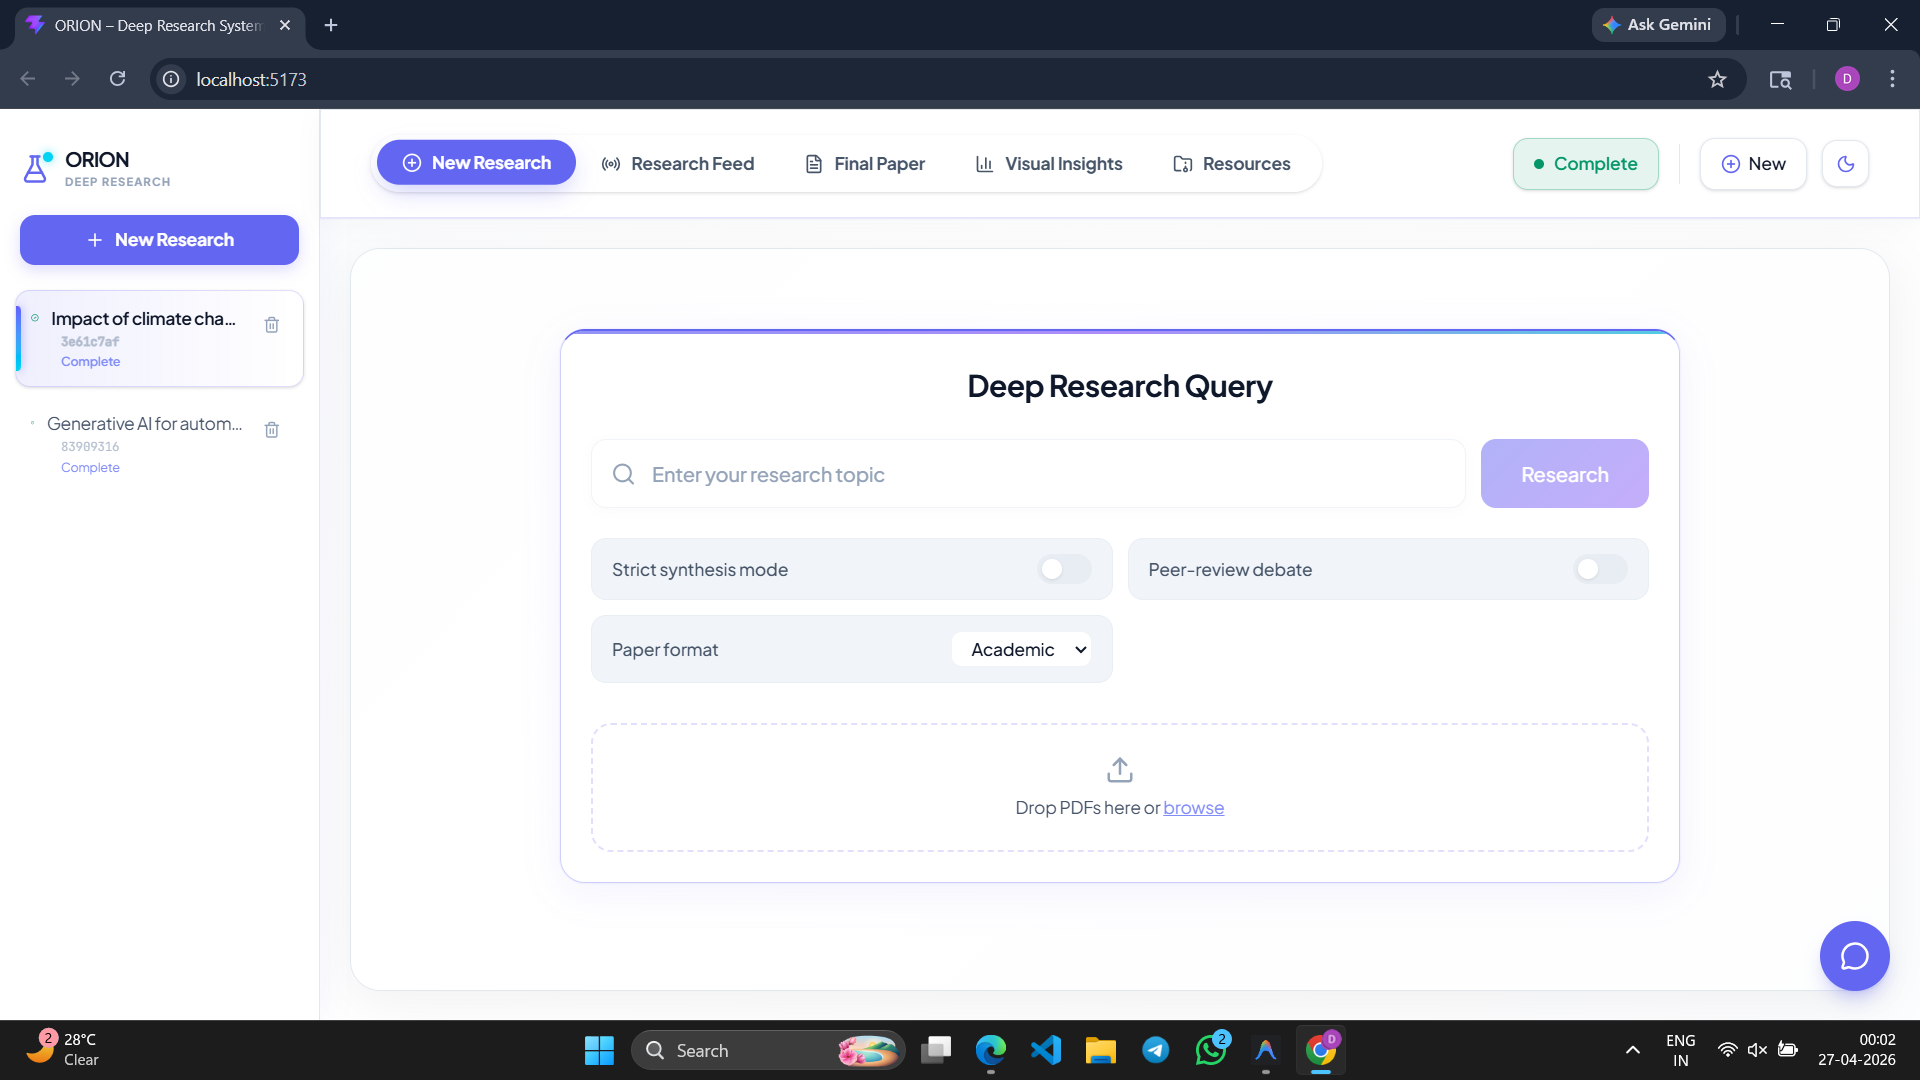
\includegraphics[width=0.88\textwidth]{ss/screenshot_71.png}
    \caption{ORION Dashboard showing Pipeline Progress and 8-Stage Node Tracker}
\end{figure}

\begin{figure}[H]
    \centering
    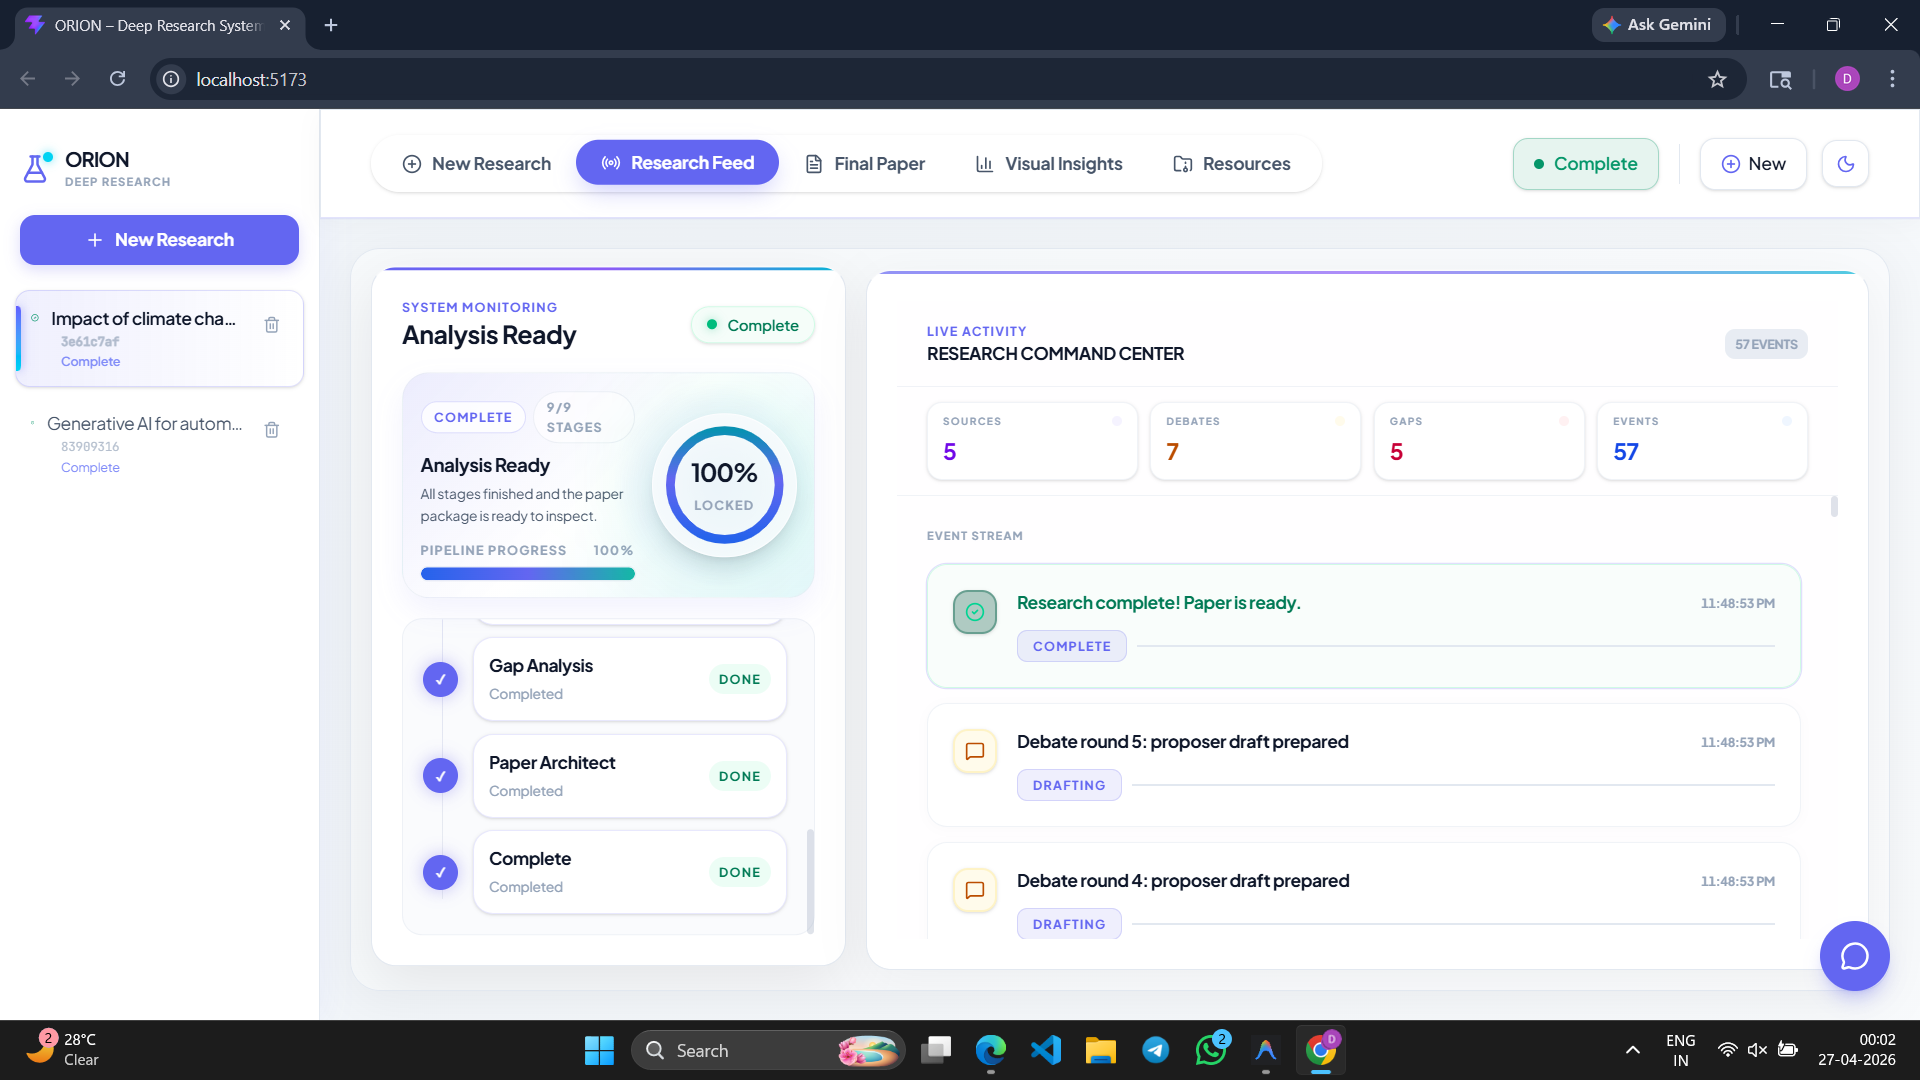
\includegraphics[width=0.88\textwidth]{ss/screenshot_72.png}
    \caption{Live Activity Feed showing real-time Agent Event Stream}
\end{figure}

\begin{figure}[H]
    \centering
    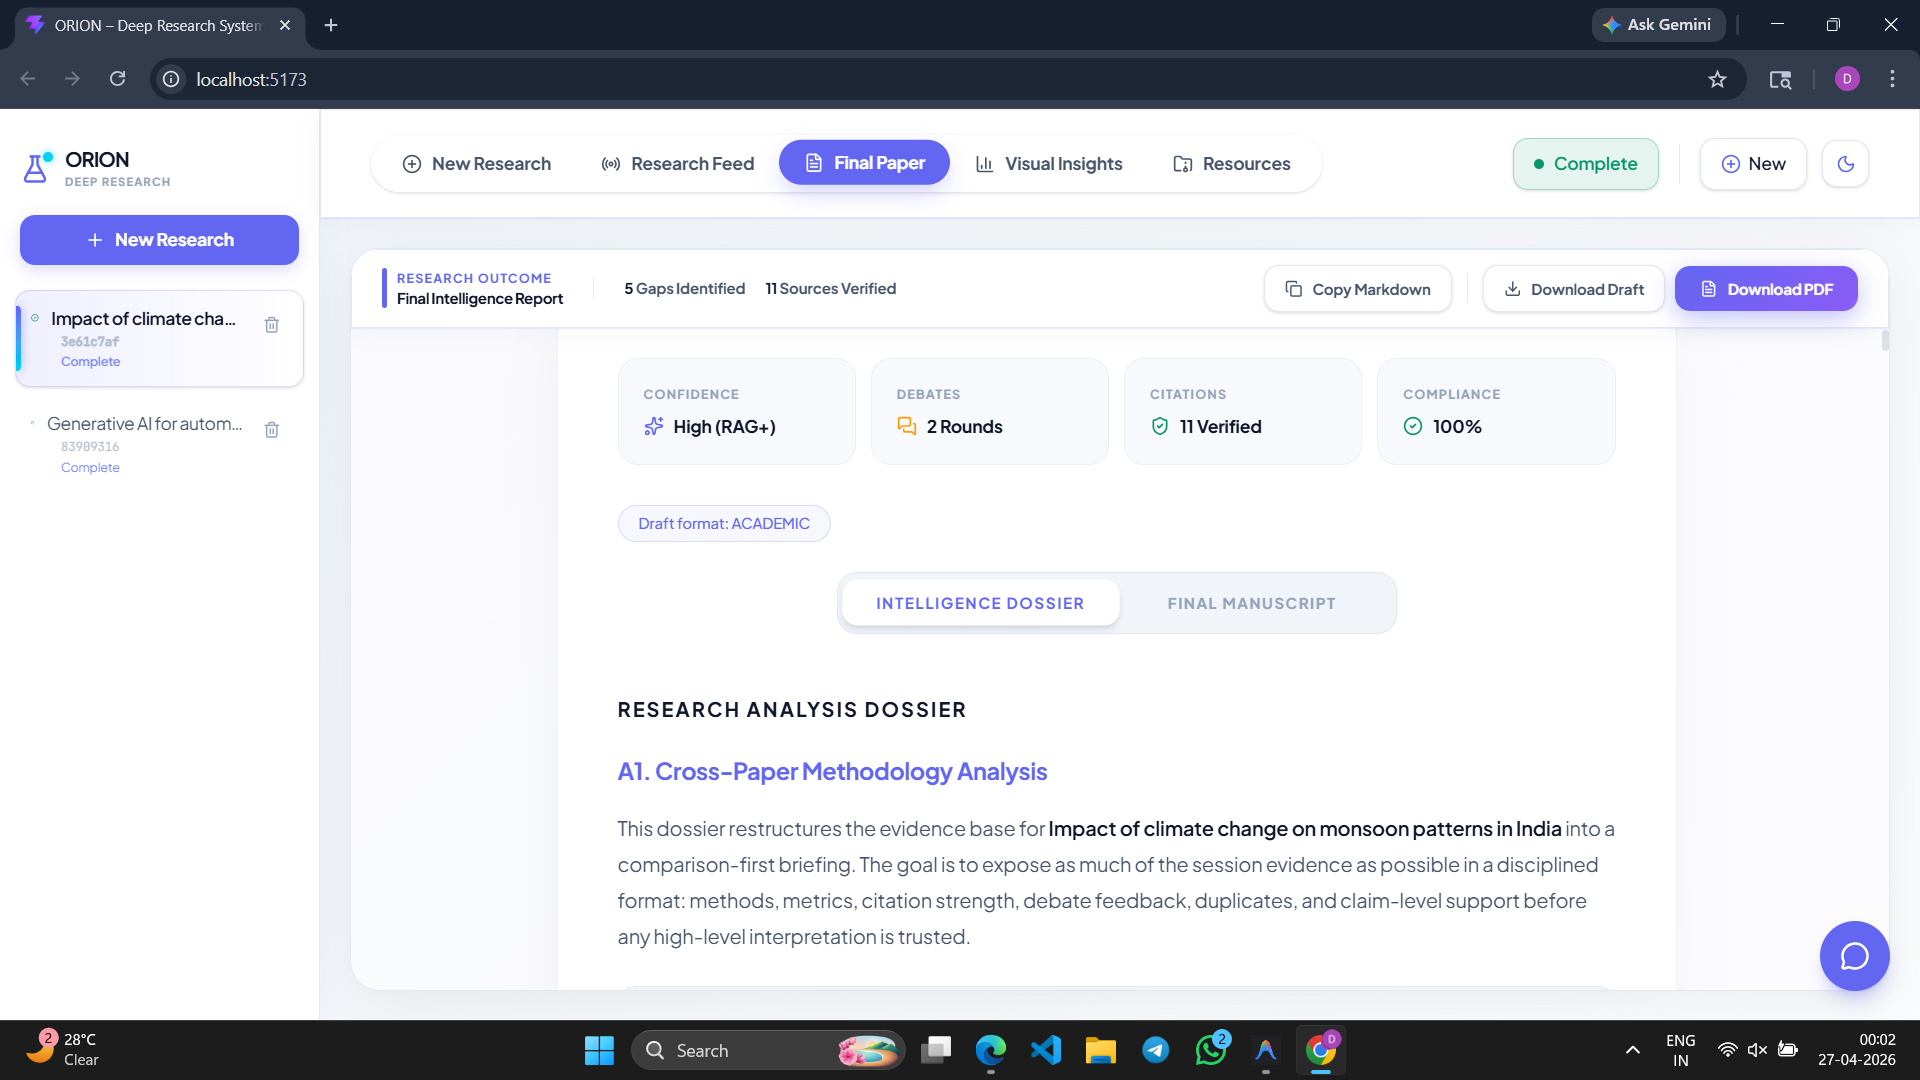
\includegraphics[width=0.88\textwidth]{ss/screenshot_73.png}
    \caption{Generated Final Paper --- Abstract and Introduction sections}
\end{figure}

\begin{figure}[H]
    \centering
    
\includegraphics[width=0.88\textwidth]{ss/screenshot_74.png}
    \caption{Cross-Paper Analysis with Methodology Breakdown and Mermaid Diagrams}
\end{figure}

\begin{figure}[H]
    \centering
    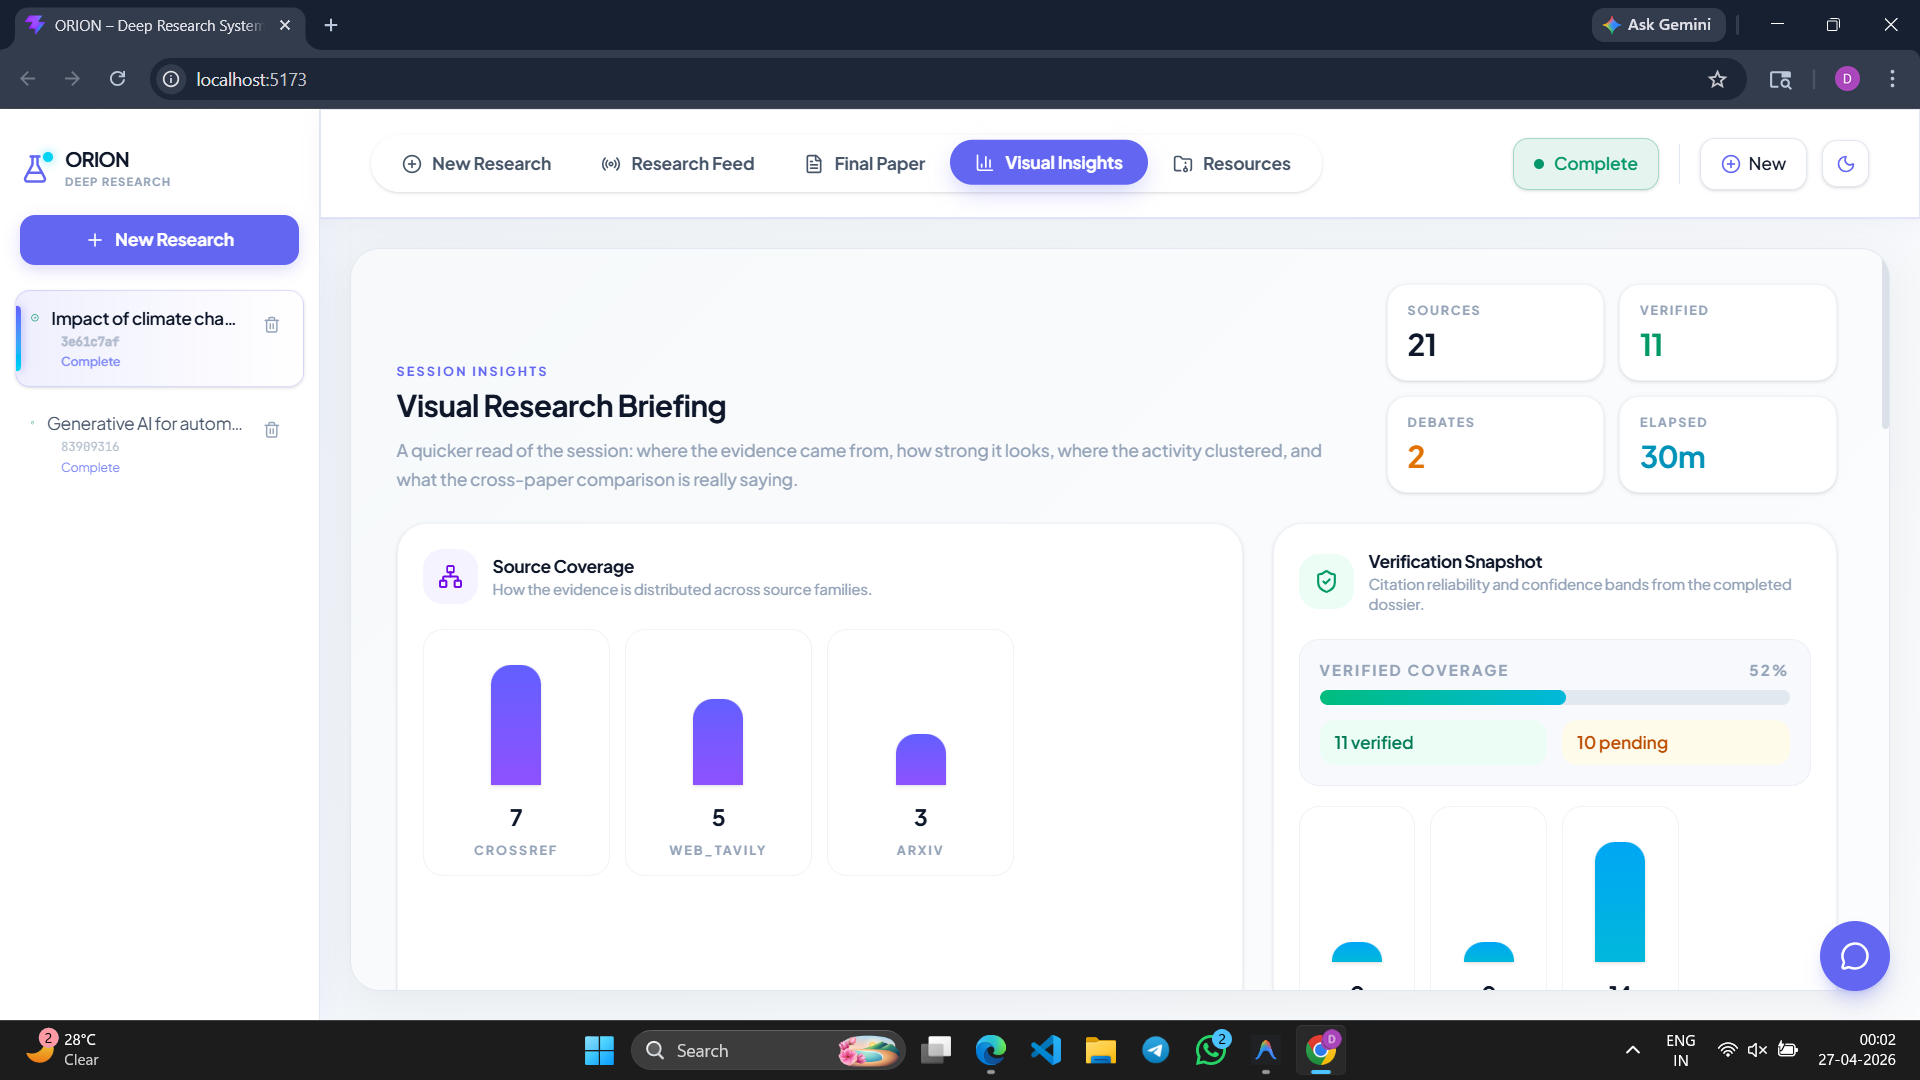
\includegraphics[width=0.88\textwidth]{ss/screenshot_75.png}
    \caption{Visual Gap Analysis Section and Structured Research Gap Cards}
\end{figure}

\begin{figure}[H]
    \centering
    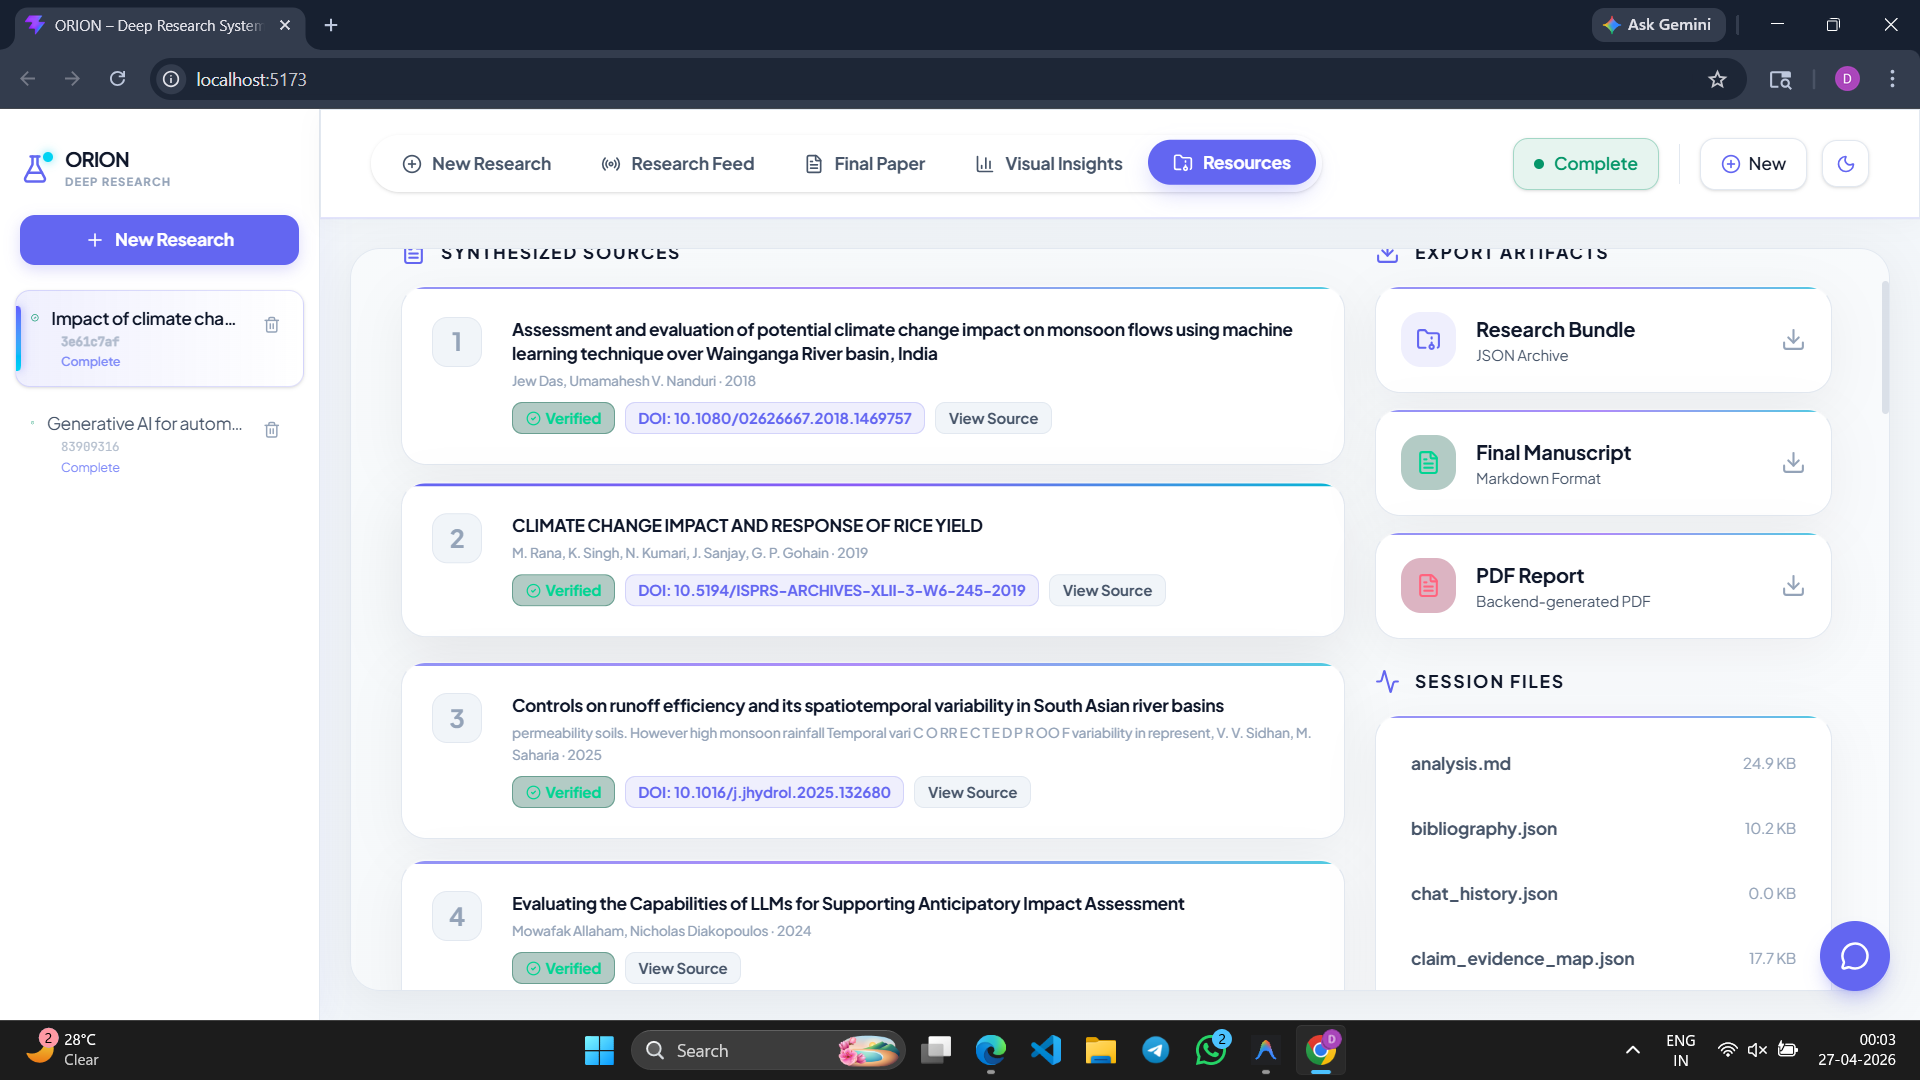
\includegraphics[width=0.88\textwidth]{ss/screenshot_76.png}
    \caption{Bibliography, Citation Verification Signals, and Format Compliance Score}
\end{figure}

%----------------------------------------------------------------------------------------
%  10. CONCLUSION
%----------------------------------------------------------------------------------------
\section{Conclusion}

The ORION Multi-Agent Deep Research Platform demonstrates the substantial potential of
graph-based LLM orchestration for academic and scientific research assistance. By decomposing
the complex task of literature review into eight specialized agentic roles and enforcing
correctness through an adversarial Critic-Proposer feedback loop, the system consistently
produces structured, well-cited, actionable research reports with a significantly lower rate
of unsupported claims compared to single-prompt LLM baselines.

The platform successfully bridges the gap between raw data retrieval and structured knowledge
synthesis, reducing a process that traditionally requires days of manual effort to a fully
automated workflow completed in minutes. The enforced citation grounding mechanism represents
a meaningful step toward trustworthy AI-assisted research, though further work is needed to
formalize citation verification beyond metadata-level heuristics.

%----------------------------------------------------------------------------------------
%  11. FUTURE SCOPE
%----------------------------------------------------------------------------------------
\section{Future Scope}

\begin{itemize}[leftmargin=*, itemsep=5pt]
    \item \textbf{Enhanced PDF Corpus Processing:} Deeper integration of OCR pipelines to
          handle scanned documents, embedded figures, and data tables within uploaded papers.

    \item \textbf{Data Analytics Agent:} A code-interpreter node capable of downloading
          datasets cited in retrieved papers and executing statistical replication scripts,
          enabling empirical validation of reported results.

    \item \textbf{Human-in-the-Loop Collaboration:} A multi-user workspace where researchers
          can intervene, annotate, and co-edit drafts during the Critic-Proposer loop,
          blending AI synthesis with domain expertise.

    \item \textbf{Domain-Specific Adaptation:} Fine-tuning or prompt specialization on
          domain corpora (medical, legal, engineering) to improve precision on highly
          specialized literature surveys.

    \item \textbf{Citation Graph Visualization:} Interactive citation network graphs rendered
          within the UI, allowing researchers to explore inter-paper relationships visually.

    \item \textbf{Formal Citation Validation:} Integration with CrossRef's metadata
          resolution API to perform bibliographic-level verification of generated references,
          moving beyond heuristic confidence flags.
\end{itemize}

%----------------------------------------------------------------------------------------
%  12. REFERENCES
%----------------------------------------------------------------------------------------
\begin{thebibliography}{99}

\bibitem{brown2020gpt}
T.\ Brown et al., ``Language models are few-shot learners,''
\textit{Advances in Neural Information Processing Systems (NeurIPS)}, vol.~33,
pp.~1877--1901, 2020.

\bibitem{ji2023hallucination}
Z.\ Ji et al., ``Survey of hallucination in natural language generation,''
\textit{ACM Computing Surveys}, vol.~55, no.~12, pp.~1--38, 2023.

\bibitem{lewis2020rag}
P.\ Lewis et al., ``Retrieval-augmented generation for knowledge-intensive NLP tasks,''
\textit{Advances in Neural Information Processing Systems (NeurIPS)}, vol.~33,
pp.~9459--9474, 2020.

\bibitem{wu2023autogen}
Q.\ Wu et al., ``AutoGen: Enabling next-gen LLM applications via multi-agent conversation,''
\textit{arXiv preprint arXiv:2308.08155}, 2023.

\bibitem{hong2023metagpt}
S.\ Hong et al., ``MetaGPT: Meta programming for a multi-agent collaborative framework,''
\textit{arXiv preprint arXiv:2308.00352}, 2023.

\bibitem{elicit2023}
Elicit Inc., ``Elicit: The AI Research Assistant,'' 2023.
[Online]. Available: \url{https://elicit.org}

\bibitem{langgraph2024}
LangChain AI, ``LangGraph: Building Stateful Multi-Actor Applications,'' 2024.
[Online]. Available: \url{https://python.langchain.com/docs/langgraph}

\bibitem{vertexai}
Google Cloud, ``Vertex AI Gemini API Documentation,'' 2024.
[Online]. Available: \url{https://cloud.google.com/vertex-ai/docs/generative-ai}

\bibitem{fastapi}
S.\ Ram\'{i}rez, ``FastAPI: Modern, Fast Web Framework for Building APIs with Python,''
2019. [Online]. Available: \url{https://fastapi.tiangolo.com}

\bibitem{chromadb}
Chroma Inc., ``Chroma: The AI-Native Open-Source Embedding Database,'' 2023.
[Online]. Available: \url{https://www.trychroma.com}

\end{thebibliography}

\newpage

%----------------------------------------------------------------------------------------
%  13. APPENDIX
%----------------------------------------------------------------------------------------
\section{Appendix}

\subsection{Core LangGraph Architecture --- \texttt{graph.py}}

The following listing shows the complete LangGraph state machine definition, including node
registrations, sequential edges, and the conditional Critic-Proposer debate routing:

\begin{lstlisting}[language=Python,
    caption={Core LangGraph graph definition --- backend/app/core/graph.py}]
from langgraph.graph import StateGraph, END
from app.core.state import ResearchState
from app.core.agents import (
    search_planner_node,
    paper_retriever_node,
    paper_reader_node,
    cross_paper_analyzer_node,
    gap_analysis_node,
    literature_reviewer_node,
    critic_node,
    paper_architect_node,
    debate_should_continue
)

def build_research_graph() -> StateGraph:
    workflow = StateGraph(ResearchState)

    # Register all agent nodes
    workflow.add_node("search_planner",       search_planner_node)
    workflow.add_node("paper_retriever",      paper_retriever_node)
    workflow.add_node("paper_reader",         paper_reader_node)
    workflow.add_node("cross_paper_analyzer", cross_paper_analyzer_node)
    workflow.add_node("gap_analysis",         gap_analysis_node)
    workflow.add_node("literature_reviewer",  literature_reviewer_node)
    workflow.add_node("critic",               critic_node)
    workflow.add_node("paper_architect",      paper_architect_node)

    # Set pipeline entry point
    workflow.set_entry_point("search_planner")

    # Sequential edges
    workflow.add_edge("search_planner",       "paper_retriever")
    workflow.add_edge("paper_retriever",      "paper_reader")
    workflow.add_edge("paper_reader",         "cross_paper_analyzer")
    workflow.add_edge("cross_paper_analyzer", "gap_analysis")
    workflow.add_edge("gap_analysis",         "literature_reviewer")
    workflow.add_edge("literature_reviewer",  "critic")

    # Adversarial debate loop:
    # debate_should_continue() returns "continue" or "end"
    # based on round count and critic approval status.
    workflow.add_conditional_edges(
        "critic",
        debate_should_continue,
        {
            "continue": "literature_reviewer",  # re-enter debate
            "end":      "paper_architect"        # proceed to final assembly
        }
    )

    workflow.add_edge("paper_architect", END)

    return workflow.compile()
\end{lstlisting}

\subsection{ResearchState Schema}

The \texttt{ResearchState} typed dictionary carries all inter-node data throughout the
pipeline. Key fields grouped by stage:

\begin{itemize}[leftmargin=*, itemsep=2pt]
    \item \textbf{Inputs:} \texttt{topic}, \texttt{uploaded\_pdf\_ids}
    \item \textbf{Planner:} \texttt{queries}, \texttt{plan}, \texttt{strict\_mode},
          \texttt{max\_debate\_rounds}, \texttt{paper\_format}
    \item \textbf{Retriever:} \texttt{retrieved\_papers}, \texttt{vector\_results},
          \texttt{source\_counts}, \texttt{duplicate\_clusters}
    \item \textbf{Summarizer:} \texttt{paper\_summaries}, \texttt{citation\_quality},
          \texttt{citation\_verification}
    \item \textbf{Debate:} \texttt{draft\_text}, \texttt{debate\_log},
          \texttt{debate\_round}
    \item \textbf{Final:} \texttt{paper\_markdown}, \texttt{bibliography},
          \texttt{claim\_evidence\_map}, \texttt{verified\_citation\_count},
          \texttt{format\_compliance\_score}
\end{itemize}

\end{document}